\documentclass{article}


\usepackage{arxiv}

\usepackage[utf8]{inputenc} 
\usepackage[T1]{fontenc}    
\usepackage{hyperref}       
\usepackage{url}            
\usepackage{booktabs}       
\usepackage{amsfonts}       
\usepackage{nicefrac}
\usepackage{graphicx}
\usepackage{subcaption}
\usepackage{verbatim}
\usepackage{adjustbox}
\usepackage{float}
\usepackage[spanish]{babel}
\usepackage{microtype}      
\usepackage{lipsum}
\usepackage{graphicx}
\usepackage{amsmath}
\graphicspath{ {./images/} }
\renewcommand{\refname}{Referencias}
\usepackage{caption}


\title{TP 1.2 - Estudio económico-matemático de apuestas en la ruleta }


\author{
 Aldana Risso Patrón \\
  Universidad Tecnológica Nacional - FRRO \\
  Zeballos 1341, S2000, Argentina \\
  \texttt{rissopatronaldana7@gmail.com} \\
   \And
 Ignacio Fierro \\
  Universidad Tecnológica Nacional - FRRO \\
  Zeballos 1341, S2000, Argentina \\
  \texttt{nachofier@gmail.com} \\
  \And
 Lucía Gelmetti \\
  Universidad Tecnológica Nacional - FRRO \\
  Zeballos 1341, S2000, Argentina \\
  \texttt{luligelmetti@gmail.com} \\
  \And
 Juan Cruz Bonanno \\
  Universidad Tecnológica Nacional - FRRO \\
  Zeballos 1341, S2000, Argentina \\
  \texttt{bonanno2340@gmail.com} \\
  \And
 Franco Reggiardo Chuglar \\
  Universidad Tecnológica Nacional - FRRO\\
  Zeballos 1341, S2000, Argentina \\
  \texttt{francoreggiardo15@gmail.com} \\
  \And
 Marcos Oldani \\
  Universidad Tecnológica Nacional - FRRO \\
  Zeballos 1341, S2000, Argentina \\
  \texttt{marcosoldani1360@gmail.com} \\
}

\begin{document}
\maketitle
\begin{abstract}
El siguiente informe tiene por objetivo profundizar en el comportamiento de la ruleta, visto del punto de vista del apostador. Incorporamos estrategias y capital, analizando los distintos resultados de cada situación.
\end{abstract}

\keywords{Simulación \and Ruleta \and Análisis Estadístico \and Martingala \and Paroli \and D'Alembert \and Fibonacci}

\section{Introducción}
En el ultimo trabajo concluimos que, si bien las corridas individuales presentan fluctuaciones en la frecuencia de aparicion de los numeros, los resultados tienden a estabilizarse al aumentar el numero de tiradas. 

Ahora, ¿cómo se comportarán los datos al añadirle nuevas variables? Para analizar esto sumamos dos variables. Por un lado la estrategia, de la cual analizamos tres tipos (Martingala, D'Alembert y Fibonacci) propuestos por la cátedra y uno (Paroli) de nuestra elección. Por otro lado la adición del capital, con la posibilidad de ser finito o infinito.

Nuestro objetivo será ver cómo se comporta el capital en la simulación con cada estrategia, y comprobar si es posible tener ventaja ante la casa de apuestas.


\section{Sistemas de Apuestas}
\subsection{D'Alembert}
En el mundo de los juegos de azar, la ruleta se erige como uno de los pasatiempos más populares y emocionantes. Entre las diversas estrategias para aumentar las probabilidades de éxito, el método D'Alembert destaca por su simplicidad y enfoque conservador.

Desarrollado en el siglo XVIII por el matemático francés Jean-Baptiste le Rond d'Alembert, este sistema de apuestas se basa en la idea de progresión lineal, ajustando las apuestas en función del resultado de las jugadas anteriores.

A diferencia de estrategias más agresivas como la Martingala, el método D'Alembert busca minimizar el riesgo y maximizar las ganancias a largo plazo, apelando a la ley de los promedios.

\subsubsection{Funcionamiento del método D'Alembert}

La estrategia D'Alembert se aplica en apuestas con probabilidades iguales, como rojo/negro, par/impar, 1-18/19-36. El jugador define una apuesta base, que representa la cantidad inicial a invertir en cada jugada.

En caso de perder:

\begin{itemize}
    \item Se incrementa la apuesta en una unidad. Esto significa que en la siguiente jugada se apostará la cantidad de la apuesta base más una unidad adicional.
\end{itemize}

En caso de ganar:

\begin{itemize}
    \item Se reduce la apuesta en una unidad. En la siguiente jugada, se apostará la cantidad de la apuesta base menos una unidad.
\end{itemize}

\textbf{Ejemplo práctico:}

\begin{itemize}
    \item Apuesta base: \$10
    \item Primera jugada: Rojo (pierde)
    \item Segunda jugada: \$10 + \$1 = \$11 (apuesta al negro)
    \item Segunda jugada: Negro (gana)
    \item Tercera jugada: \$11 - \$1 = \$10 (apuesta al rojo)
\end{itemize}

\subsubsection{Consideraciones importantes:}

\begin{itemize}
    \item Establecimiento de límites: Es fundamental definir un límite de pérdidas y un límite de ganancias para cada sesión de juego. Esto permite un control del bankroll y evita emociones que puedan afectar la toma de decisiones.
    \item Gestión del bankroll: La estrategia D'Alembert no garantiza ganancias a corto plazo. Es crucial administrar el bankroll de manera responsable, apostando solo una pequeña porción del mismo en cada jugada.
    \item Probabilidades y azar: Es importante recordar que la ruleta es un juego de azar y que el casino siempre tiene una ventaja. El método D'Alembert puede ayudar a gestionar el riesgo, pero no elimina la posibilidad de perder.
\end{itemize}

\subsubsection{Ventajas y desventajas del método D'Alembert}

\textbf{Ventajas:}

\begin{itemize}
    \item Simplicidad: Su facilidad de comprensión y aplicación lo convierte en un método accesible para jugadores de todos los niveles.
    \item Bajo riesgo: Al aumentar las apuestas de forma gradual, se minimiza el riesgo de perder grandes sumas de dinero en una sola jugada.
    \item Potencial de ganancias a largo plazo: La estrategia busca aprovechar las rachas de victorias para recuperar pérdidas y obtener ganancias consistentes.
\end{itemize}

\textbf{Desventajas:}

\begin{itemize}
    \item Progreso lento: Las ganancias pueden ser graduales y requerir un número considerable de jugadas para obtener resultados significativos.
    \item No elimina la ventaja del casino: Al igual que cualquier estrategia de apuestas, no elimina la ventaja matemática que siempre tiene el casino.
    \item Dependencia de las rachas: El éxito del método depende en gran medida de la capacidad del jugador para aprovechar las rachas de victorias.
\end{itemize}

La estrategia de apuestas en la ruleta de D'Alembert se presenta como una opción viable para aquellos jugadores que buscan un enfoque metódico y conservador. Su simplicidad, bajo riesgo y potencial de ganancias a largo plazo la convierten en una alternativa atractiva para quienes buscan disfrutar del juego de forma responsable.

Es importante recordar que, si bien el método puede ayudar a gestionar el bankroll y aumentar las probabilidades de éxito, no existe una fórmula mágica que garantice ganancias en el juego de azar. La clave reside en la disciplina, la gestión responsable del dinero y la comprensión de las probabilidades inherentes a la ruleta.

\subsection{Paroli}
Esta estrategia se basa en la hipótesis de que las ganancias y pérdidas tienden a aparecer por rachas, por lo tanto, Paroli busca aprovechar las rachas de ganancia al máximo. 

Su nombre se deriva del término latino par, que significa “uno igual". Desde el siglo XVI que se lleva empleado para diferentes propósitos, pero el más popular hoy en día es la ya conocida ruleta, por lo que vamos a simular su funcionamiento a continuación.

\subsubsection{Funcionamiento del método Paroli}

La estrategia consiste en apostar siempre lo mismo cuando se pierde, y aumentar la apuesta cuando se gana, pero a diferencia de la estrategia Martingala de la que se hablará mas adelante, este aumento sólo se realiza hasta ganar tres veces seguidas. Así se aplica el pensamiento de que las ganancias aparecen por rachas. Cuando se gana por tercera vez consecutiva, se vuelve a apostar la cantidad inicial.

En caso de ganar:

\begin{itemize}
    \item Si no es la tercera vez consecutiva que se acierta, se duplica la apuesta. Caso contrario, se vuelve a la apuesta inicial.
\end{itemize}

En caso de perder:

\begin{itemize}
    \item Se apuesta la cantidad inicial.
\end{itemize}

\textbf{Ejemplo práctico:}

\begin{itemize}
    \item Apuesta base: \$10
    \item Primera jugada: Rojo (pierde)
    \item Segunda jugada: \$10 (apuesta al rojo)
    \item Segunda jugada: Rojo (gana)
    \item Tercera jugada: \$20 (apuesta al rojo)
    \item Tercera jugada: Rojo (gana)
    \item Cuarta jugada: \$40 (apuesta al rojo)
    \item Cuarta jugada: Rojo (gana)
    \item Quinta jugada: \$80 (apuesta al rojo)
    \item Quinta jugada: Rojo (gana)
    \item Sexta jugada: \$10 (apuesta al rojo)
    \item Sexta jugada: Negro (pierde)
\end{itemize}

\subsubsection{Consideraciones importantes:}

\begin{itemize}
    \item Establecimiento de límites: Es fundamental definir un límite de ganancias y un límite de pérdidas para cada sesión de juego. Esto permite un control del bankroll y evita emociones que puedan afectar la toma de decisiones.
    \item Gestión del bankroll: La estrategia Paroli no garantiza ganancias a corto plazo. Es crucial administrar el bankroll de manera responsable, apostando solo una pequeña porción del mismo en cada jugada.
    \item Probabilidades y azar: Es importante recordar que la ruleta es un juego de azar y que el casino siempre tiene una ventaja. El método Paroli puede ayudar a maximizar las ganancias durante rachas positivas, pero no elimina la posibilidad de perder.
\end{itemize}

\subsubsection{Ventajas y desventajas del método Paroli}

\textbf{Ventajas:}

\begin{itemize}
    \item Potencial de ganancias elevadas: Al duplicar las apuestas en rachas de victorias, se pueden obtener ganancias significativas en un corto período de tiempo.
    \item Simplicidad: Su facilidad de comprensión y aplicación lo convierte en un método accesible para jugadores de todos los niveles.
    \item Aprovechamiento de rachas: La estrategia busca capitalizar las rachas de victorias, lo que puede ser beneficioso en ciertos momentos del juego.
\end{itemize}

\textbf{Desventajas:}

\begin{itemize}
    \item Alto riesgo: Al aumentar las apuestas de forma exponencial, se incrementa significativamente el riesgo de perder grandes sumas de dinero en una sola jugada.
    \item Dependencia de las rachas: El éxito del método depende en gran medida de la capacidad del jugador para experimentar rachas de victorias consecutivas.
    \item Limitaciones del bankroll: La estrategia puede ser inviable para jugadores con un bankroll limitado, ya que requiere duplicar las apuestas en cada victoria.
\end{itemize}

\subsubsection{Formalización matemática}

Sea $X_n$ la variable aleatoria que representa el resultado de la jugada $n$, donde:

\[ X_n = \begin{cases} 
1 & \text{si se gana en la jugada } n \\
-1 & \text{si se pierde en la jugada } n 
\end{cases} \]

La apuesta para la jugada $n+1$ se define como:

\[ A_{n+1} = A_n \cdot 2^{nv_{n-1}} \]

Donde:

$A_{n+1}$ es la apuesta para la jugada $n+1$ \\
$A_n$ es la apuesta para la jugada $n$ \\
$nv_{n-1}$ es el número de victorias consecutivas hasta la jugada $n-1$ \\
En el caso del método Paroli, $nv_{n-1} = 1$ si se ganó en la jugada $n-1$ y $nv_{n-1} = 0$ si se perdió en la jugada $n-1$. 

\subsection{Martingala}
En el ámbito de los juegos de azar, la estrategia Martingala se posiciona como una técnica popular, reconocida por su simplicidad y enfoque audaz. A diferencia de métodos conservadores como D'Alembert o Paroli, la Martingala apuesta por recuperar las pérdidas de manera expeditiva, duplicando la apuesta tras cada jugada perdida.

Desarrollada en el siglo XVII en Francia, esta estrategia se basa en la idea de que, a largo plazo, las ganancias deberían igualar o superar las pérdidas, siempre que el jugador cuente con fondos suficientes para cubrir las apuestas crecientes.

\subsubsection{Funcionamiento del método Martingala}

La estrategia Martingala se aplica en apuestas con probabilidades iguales, como rojo/negro, par/impar, 1-18/19-36. El jugador define una apuesta base, que representa la cantidad inicial a invertir en cada jugada.

En caso de perder:

\begin{itemize}
    \item Se duplica la apuesta en la siguiente jugada.
\end{itemize}

En caso de ganar:

\begin{itemize}
    \item Se regresa a la apuesta base en la siguiente jugada.
\end{itemize}

\textbf{Ejemplo práctico:}

\begin{itemize}
    \item Apuesta base: \$10
    \item Primera jugada: Rojo (pierde)
    \item Segunda jugada: \$20 (apuesta al rojo)
    \item Segunda jugada: Rojo (pierde)
    \item Tercera jugada: \$40 (apuesta al rojo)
    \item Tercera jugada: Rojo (gana)
    \item Cuarta jugada: \$10 (apuesta base)
\end{itemize}

\subsubsection{Consideraciones importantes:}

\begin{itemize}
    \item Establecimiento de límites: Es fundamental definir un límite de pérdidas para cada sesión de juego. Esto permite un control del bankroll y evita emociones que puedan afectar la toma de decisiones.
    \item Gestión del bankroll: La estrategia Martingala no garantiza ganancias a corto plazo. Es crucial administrar el bankroll de manera responsable, apostando solo una pequeña porción del mismo en cada jugada.
    \item Probabilidades y azar: Es importante recordar que la ruleta es un juego de azar y que el casino siempre tiene una ventaja. El método Martingala puede ayudar a recuperar pérdidas en el corto plazo, pero no elimina la posibilidad de perder a largo plazo.
\end{itemize}

\subsubsection{Ventajas y desventajas del método Martingala}

\textbf{Ventajas:}

\begin{itemize}
    \item Simplicidad: Su facilidad de comprensión y aplicación lo convierte en un método accesible para jugadores de todos los niveles.
    \item Potencial de recuperación rápida: Al duplicar las apuestas en jugadas perdidas, se puede recuperar el dinero perdido en un corto período de tiempo.
    \item Aprovechamiento de rachas: La estrategia busca capitalizar las rachas de victorias, lo que puede ser beneficioso en ciertos momentos del juego.
\end{itemize}

\textbf{Desventajas:}

\begin{itemize}
    \item Alto riesgo: El aumento exponencial de las apuestas implica un riesgo considerable de perder grandes sumas de dinero en una sola jugada.
    \item Dependencia del bankroll: La estrategia requiere un bankroll significativo para soportar las duplicaciones de apuestas, lo que puede ser un obstáculo para algunos jugadores.
    \item Probabilidades desfavorables: A largo plazo, la ventaja matemática del casino siempre prevalecerá, haciendo que la Martingala sea una estrategia insostenible.
\end{itemize}

\subsubsection{Formalización matemática}

Sea $X_n$ la variable aleatoria que representa el resultado de la jugada $n$, donde:

\[ X_n = \begin{cases} 
1 & \text{si se gana en la jugada } n \\
-1 & \text{si se pierde en la jugada } n 
\end{cases} \]

La apuesta para la jugada $n+1$ se define como:

\[ A_{n+1} = A_n \cdot 2^{nd_{n-1}} \]

Donde:

$A_{n+1}$ es la apuesta para la jugada $n+1$ \\
$A_n$ es la apuesta para la jugada $n$ \\
$nd_{n-1}$ es el número de derrotas consecutivas hasta la jugada $n-1$ \\
En el caso del método Martingala, $nd_{n-1} = 1$ si se perdió en la jugada $n-1$ y $nd_{n-1} = 0$ si se ganó en la jugada $n-1$.

\subsection{Fibonacci}
En el mundo de las apuestas en la ruleta, la estrategia Fibonacci se presenta como una alternativa que busca minimizar el riesgo y maximizar las ganancias a largo plazo, inspirándose en la famosa secuencia matemática. A diferencia de métodos agresivos como la Martingala, Fibonacci apuesta por aumentar las apuestas de forma gradual siguiendo la sucesión de Fibonacci, y reducirlas en caso de ganar.

Desarrollada en el siglo XIII por el matemático italiano Leonardo de Pisa, conocido como Fibonacci, esta estrategia se basa en la idea de progresión y equilibrio, buscando aprovechar las rachas de victorias y minimizar las pérdidas.

\subsubsection{Funcionamiento del método Fibonacci}

La estrategia Fibonacci se aplica en apuestas con probabilidades iguales, como rojo/negro, par/impar, 1-18/19-36. El jugador define una apuesta base, que representa la cantidad inicial a invertir en cada jugada.

En caso de perder:

\begin{itemize}
    \item Se incrementa la apuesta siguiendo la secuencia de Fibonacci. Esto significa que en la siguiente jugada se apostará la cantidad de la apuesta base más la cantidad de la jugada anterior.
\end{itemize}

En caso de ganar:

\begin{itemize}
    \item Se retrocede dos pasos en la secuencia de Fibonacci. En la siguiente jugada, se apostará la cantidad de la apuesta base menos dos posiciones en la secuencia.
\end{itemize}

\textbf{Ejemplo práctico:}

\begin{itemize}
    \item Apuesta base: $1$
    \item Secuencia de Fibonacci: $1, 1, 2, 3, 5, 8, 13, 21, 34, 55, 89, 144, 233, 377, 610, \ldots$
    \item Primera jugada: Rojo (pierde)
    \item Segunda jugada: $1 + 1 = 2$ (apuesta al rojo)
    \item Segunda jugada: Rojo (pierde)
    \item Tercera jugada: $2 + 1 = 3$ (apuesta al rojo)
    \item Tercera jugada: Rojo (gana)
    \item Cuarta jugada: $3 - 2 = 1$ (apuesta al rojo)
\end{itemize}

\subsubsection{Consideraciones importantes:}

\begin{itemize}
    \item Establecimiento de límites: Es fundamental definir un límite de pérdidas y un límite de ganancias para cada sesión de juego. Esto permite un control del bankroll y evita emociones que puedan afectar la toma de decisiones.
    \item Gestión del bankroll: La estrategia Fibonacci no garantiza ganancias a corto plazo. Es crucial administrar el bankroll de manera responsable, apostando solo una pequeña porción del mismo en cada jugada.
    \item Probabilidades y azar: Es importante recordar que la ruleta es un juego de azar y que el casino siempre tiene una ventaja. El método Fibonacci puede ayudar a gestionar el riesgo y aumentar las probabilidades de éxito, pero no elimina la posibilidad de perder.
\end{itemize}

\subsubsection{Ventajas y desventajas del método Fibonacci}

\textbf{Ventajas:}

\begin{itemize}
    \item Simplicidad: Su facilidad de comprensión y aplicación lo convierte en un método accesible para jugadores de todos los niveles.
    \item Bajo riesgo: Al aumentar las apuestas de forma gradual, se minimiza el riesgo de perder grandes sumas de dinero en una sola jugada.
    \item Potencial de ganancias a largo plazo: La estrategia busca aprovechar las rachas de victorias para recuperar pérdidas y obtener ganancias consistentes.
\end{itemize}

\textbf{Desventajas:}

\begin{itemize}
    \item Progreso lento: Las ganancias pueden ser graduales y requerir un número considerable de jugadas para obtener resultados significativos.
    \item No elimina la ventaja del casino: Al igual que cualquier estrategia de apuestas, no elimina la ventaja matemática que siempre tiene el casino.
    \item Dependencia de las rachas: El éxito del método depende en gran medida de la capacidad del jugador para aprovechar las rachas de victorias.
\end{itemize}

\subsubsection{Formalización matemática}

Sea $X_n$ la variable aleatoria que representa el resultado de la jugada $n$, donde:

\[ X_n = \begin{cases} 
1 & \text{si se gana en la jugada } n \\
-1 & \text{si se pierde en la jugada } n 
\end{cases} \]

La apuesta para la jugada $n+1$ se define como:

\[ A_{n+1} = A_n + A_{n-1} \cdot X_{n-1} \]

Donde:

$A_{n+1}$ es la apuesta para la jugada $n+1$ \\
$A_n$ es la apuesta para la jugada $n$ \\
$A_{n-1}$ es la apuesta para la jugada $n-1$ \\
En el caso del método Fibonacci, se sigue la secuencia de Fibonacci para determinar las apuestas.

\section{Ejecución de la Simulación}
\paragraph{Corridas y tiradas.} Para las ejecuciones de las simulaciones, determinamos de forma empírica un número de tiradas de 2.000, ya que antes de ese punto la mayoría de las simulaciones se detienen por bancarrota, y si el capital es infinito, demuestra el comportamiento de la estrategia a largo plazo. Ademas, se harán 5 corridas por estrategia cuando se use capital finito, y 2 corridas por estrategia con capital infinito.

\subsection{Estrategia D'Alembert}
La estrategia de D'Alembert busca recuperar pérdidas de forma progresiva, aumentando la apuesta en una unidad tras cada pérdida y reduciéndola tras una ganancia. Esta progresión lineal la convierte en una estrategia relativamente conservadora.

El gráfico de barras muestra la frecuencia relativa promedio en bloques sucesivos de tiradas. Se observa una oscilación moderada en torno al valor teórico esperado del 48.65\%, sin tendencias sistemáticas, lo que indica un comportamiento coherente con una ruleta justa.

A medida que se incrementa el número de tiradas, la frecuencia relativa acumulada tiende a estabilizarse en torno al valor teórico, en concordancia con las leyes probabilísticas, que sugieren que las proporciones observadas se acercan a las probabilidades reales con suficientes repeticiones.
\begin{figure}[H]
    \centering
    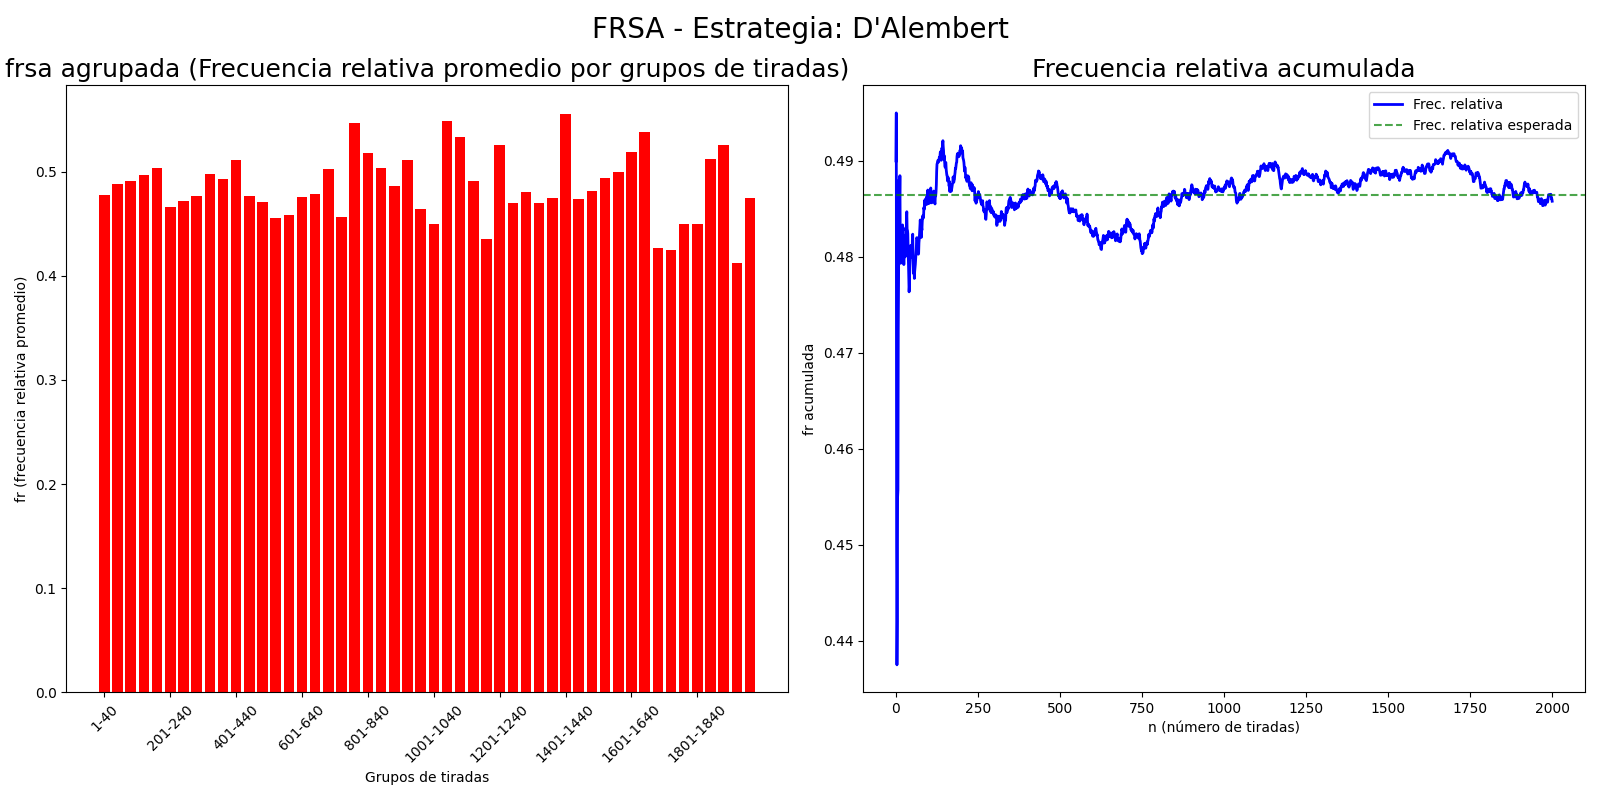
\includegraphics[width=1\textwidth]{Imagenes/frsa_D'Alembert.png}
    \caption{Frecuencia relativa promedio acumulada}
    \label{fig:dal_frsa}
\end{figure}

\begin{itemize}
    \item \textbf{Caja finita:} En este escenario, el jugador comienza con un capital limitado (100 unidades). Aunque la estrategia evita grandes apuestas iniciales, rachas prolongadas de pérdidas pueden llevar rápidamente a la banca rota. En varias simulaciones, se observó el agotamiento del capital, evidenciando la vulnerabilidad del sistema frente a la varianza del azar cuando se dispone de recursos limitados.
    \begin{figure}[H]
        \centering
        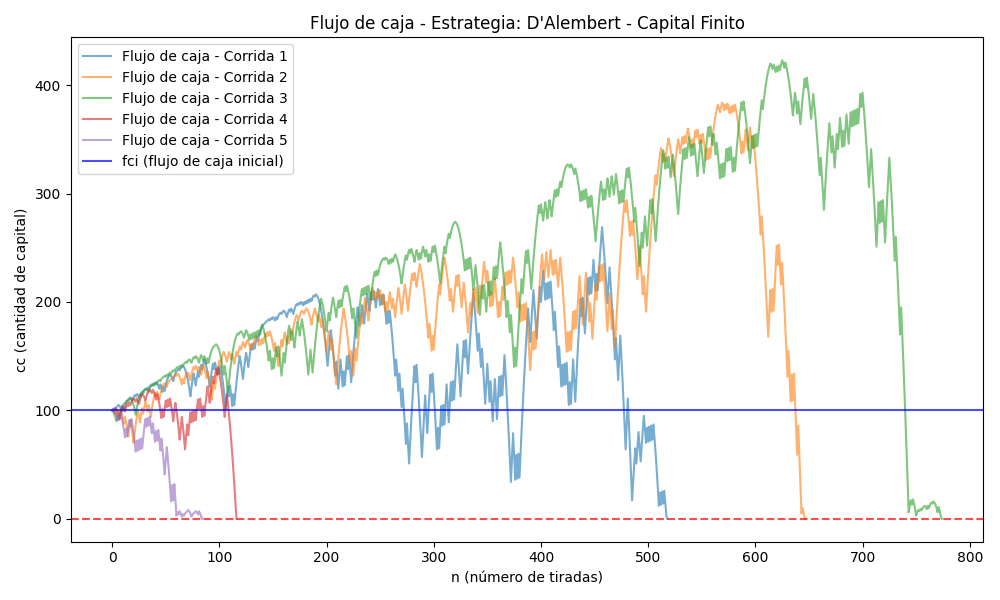
\includegraphics[width=0.7\textwidth]{Imagenes/flujo_caja_D'Alembert_f.png}
        \caption{Flujo de caja con capital finito}
        \label{fig:dal_finita}
    \end{figure}

    \item \textbf{Caja infinita:} Sin restricciones de capital, la estrategia puede mantenerse de forma indefinida. No obstante, los resultados muestran una tendencia general decreciente del capital a largo plazo. Aunque existen recuperaciones parciales, el flujo de caja tiende a disminuir debido a la ventaja matemática del casino. Esto refleja que, incluso bajo condiciones ideales, la estrategia no resulta rentable sostenidamente.
    \begin{figure}[H]
        \centering
        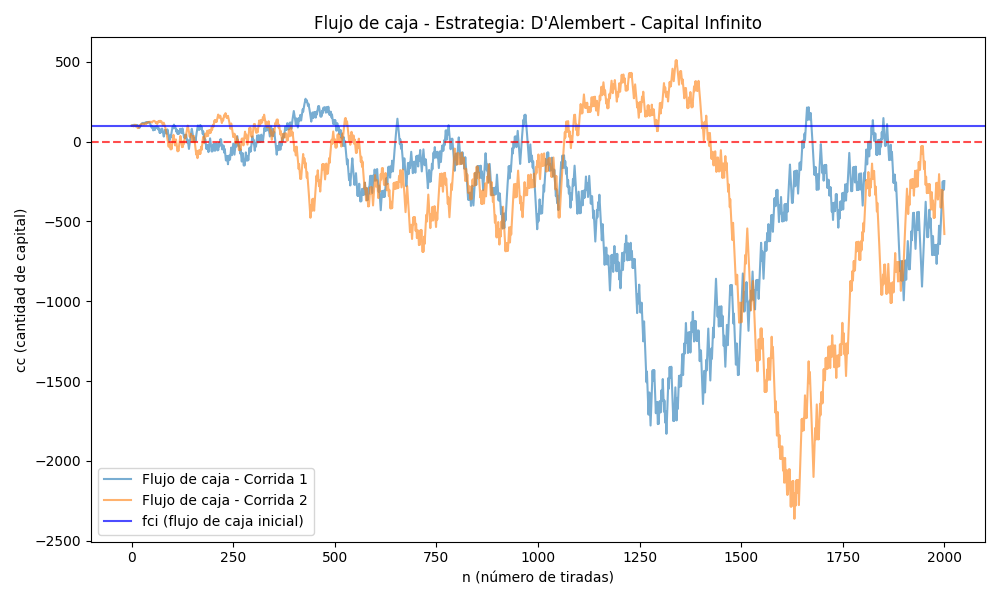
\includegraphics[width=0.7\textwidth]{Imagenes/flujo_caja_D'Alembert_i.png}
        \caption{Flujo de caja con capital infinito}
        \label{fig:dal_infinita}
    \end{figure}
\end{itemize}
    
\subsubsection{Estrategia Martingala}
La estrategia Martingala consiste en duplicar la apuesta tras cada pérdida con el objetivo de recuperar lo perdido y obtener una ganancia igual a la apuesta base. Es una de las estrategias más conocidas y agresivas dentro del ámbito de los juegos de azar.

En el análisis de frecuencias, el gráfico de barras muestra oscilaciones en torno al valor esperado del 48.65\%, reflejando la aleatoriedad característica del sistema. A medida que aumentan las tiradas, la frecuencia relativa acumulada converge gradualmente hacia ese valor, en consonancia con las leyes probabilísticas que rigen este tipo de fenómenos aleatorios.
\begin{figure}[H]
        \centering
        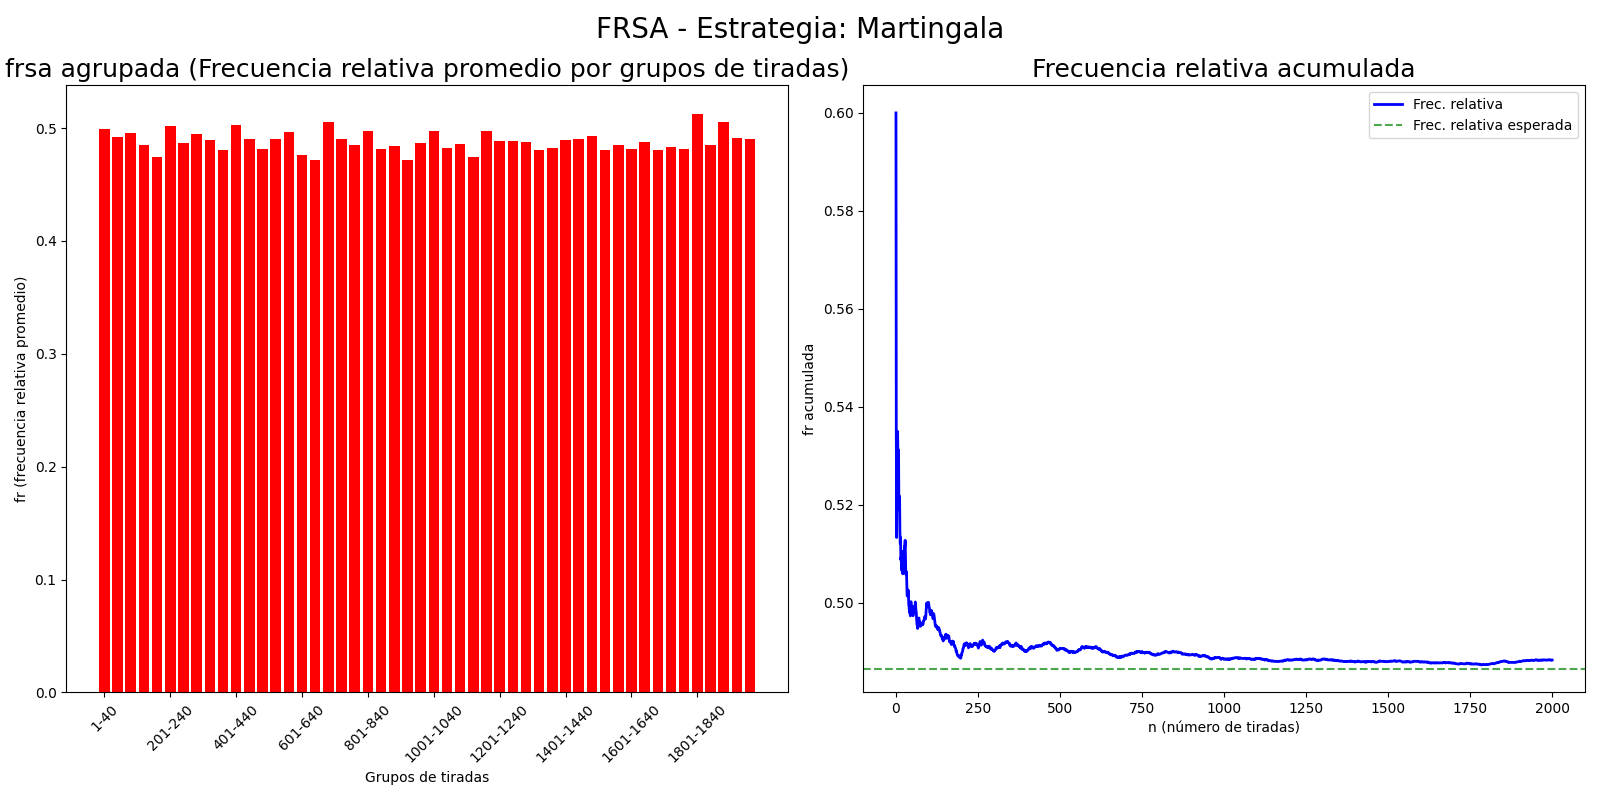
\includegraphics[width=1\textwidth]{Imagenes/frsa_Martingala.png}
        \caption{Frecuencia relativa promedio acumulada}
        \label{fig:mg_finita}    
    \end{figure}

\begin{itemize}
    \item \textbf{Caja Finita:} Con un capital inicial acotado (100 unidades), la estrategia puede generar ganancias rápidas en el corto plazo siempre que las rachas de pérdidas no sean prolongadas. Sin embargo, ante una sucesión adversa, las apuestas se duplican exponencialmente, agotando el capital en pocas jugadas. Las simulaciones evidencian esta fragilidad: varias corridas finalizan en banca rota, lo que subraya el elevado riesgo de esta estrategia en condiciones realistas con recursos limitados.
\end{itemize}
    \begin{figure}[H]
        \centering
        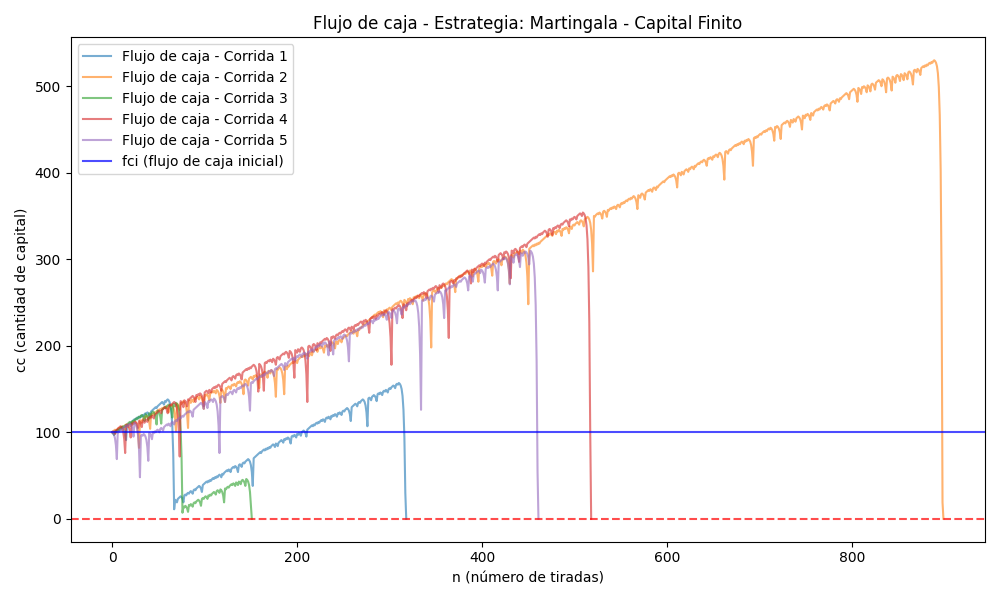
\includegraphics[width=0.7\textwidth]{Imagenes/flujo_caja_Martingala_f.png}
        \caption{Flujo de caja con capital finito}
        \label{fig:mg_finita}    
    \end{figure}
    
\begin{itemize}
    \item \textbf{Caja Infinita:} Al eliminar las restricciones de capital, la Martingala puede sostenerse indefinidamente. En este contexto ideal, el jugador eventualmente recupera sus pérdidas y obtiene beneficios. El flujo de caja tiende a ser crecientemente positivo en promedio, pero con caídas abruptas durante las rachas negativas. A pesar de los repuntes tras cada recuperación, el comportamiento no es estable ni libre de riesgos: el costo potencial de una mala racha sigue siendo muy alto. Esto confirma que, incluso en un escenario sin limitaciones financieras, la estrategia no escapa a los efectos de la ventaja estadística del casino.
\end{itemize}
    \begin{figure}[H]
        \centering
        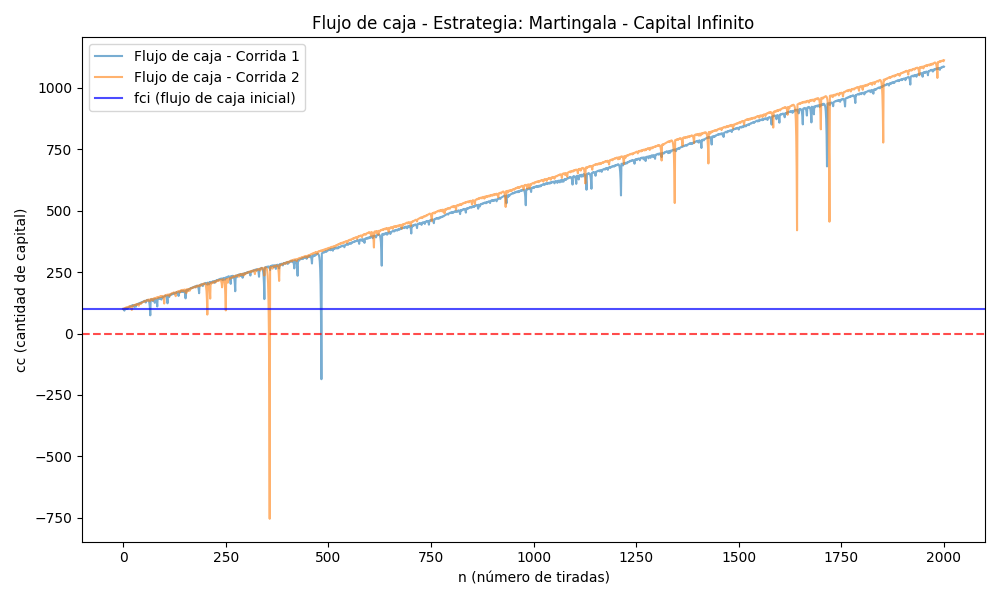
\includegraphics[width=0.7\textwidth]{Imagenes/flujo_caja_Martingala_i.png}
        \caption{Flujo de caja con capital infinito}
        \label{fig:mg_finita}    
    \end{figure}
    
\subsubsection{Estrategia de Fibonacci}
La estrategia Fibonacci se basa en una progresión matemática en la que cada número es la suma de los dos anteriores. En el ámbito de las apuestas, esta secuencia se aplica aumentando la cantidad apostada tras cada pérdida y retrocediendo dos posiciones tras una ganancia, lo que permite una progresión más controlada que estrategias más agresivas como Martingala.

En el análisis de frecuencias, el gráfico de barras presenta oscilaciones alrededor del valor teórico esperado de 48.65\%, en concordancia con el carácter aleatorio del juego. La frecuencia relativa acumulada muestra una tendencia convergente hacia ese mismo valor, cumpliendo con las expectativas probabilísticas en juegos de azar.
\begin{figure}[H]
    \centering 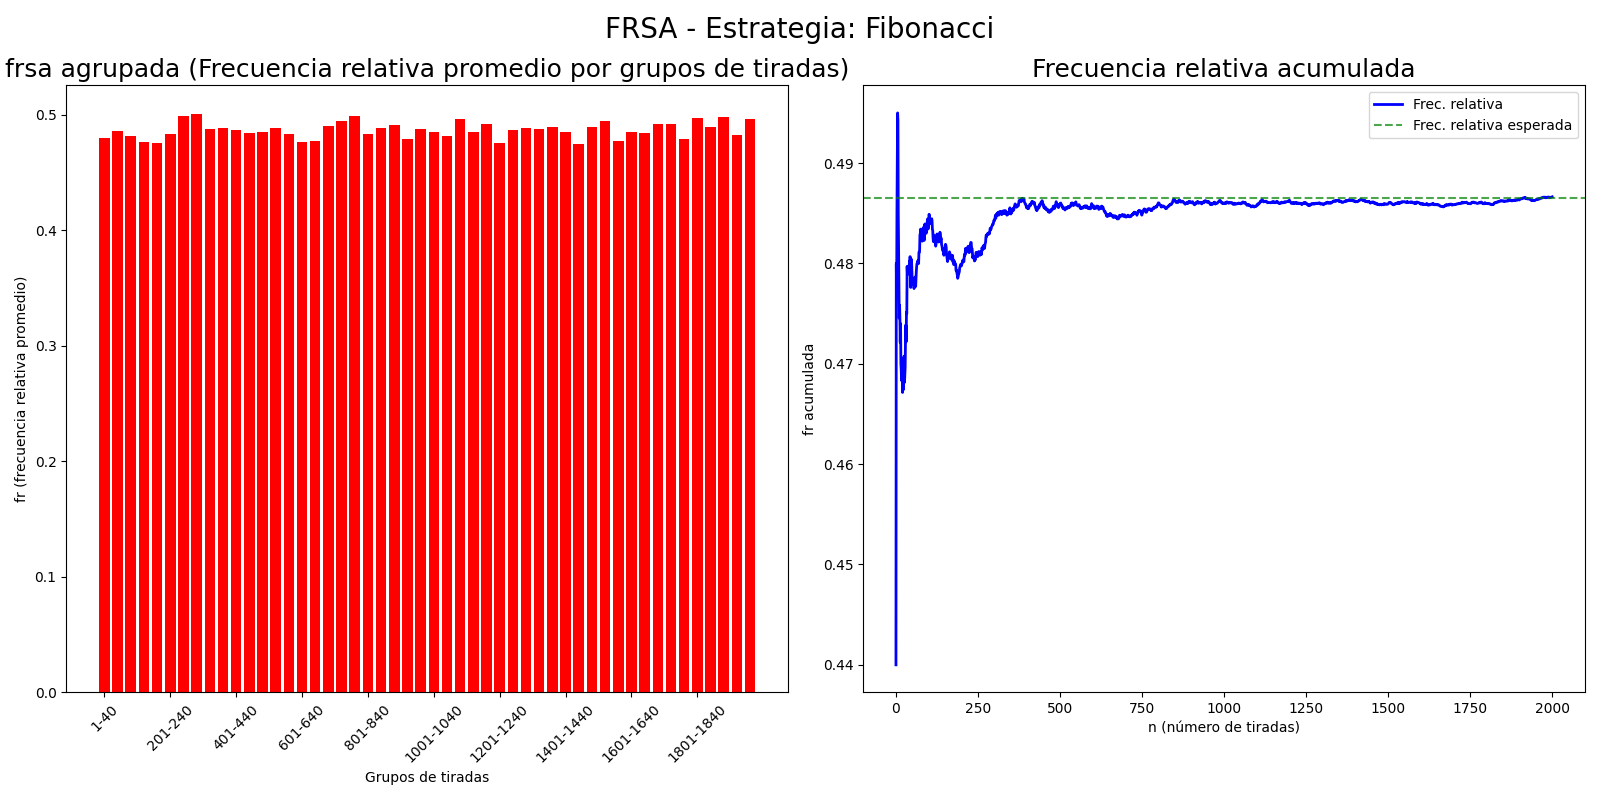
\includegraphics[width=1\linewidth]{Imagenes/frsa_Fibonacci.png}
    \caption{Frecuencia relativa promedio acumulada}
    \label{fig:enter-label}
 \end{figure}

\begin{itemize}
    \item \textbf{Caja Finita:} Con un capital inicial limitado (100 unidades), la estrategia Fibonacci demuestra un comportamiento más estable frente a rachas adversas. Gracias al incremento moderado de las apuestas, se evita una escalada agresiva del capital comprometido, como ocurre en otras estrategias. Las simulaciones muestran un flujo de caja más sostenido, sin caídas abruptas, y una menor frecuencia de bancas rotas, lo que sugiere que esta estrategia puede ser más adecuada en entornos con recursos limitados.
    \begin{figure}[H]
        \centering 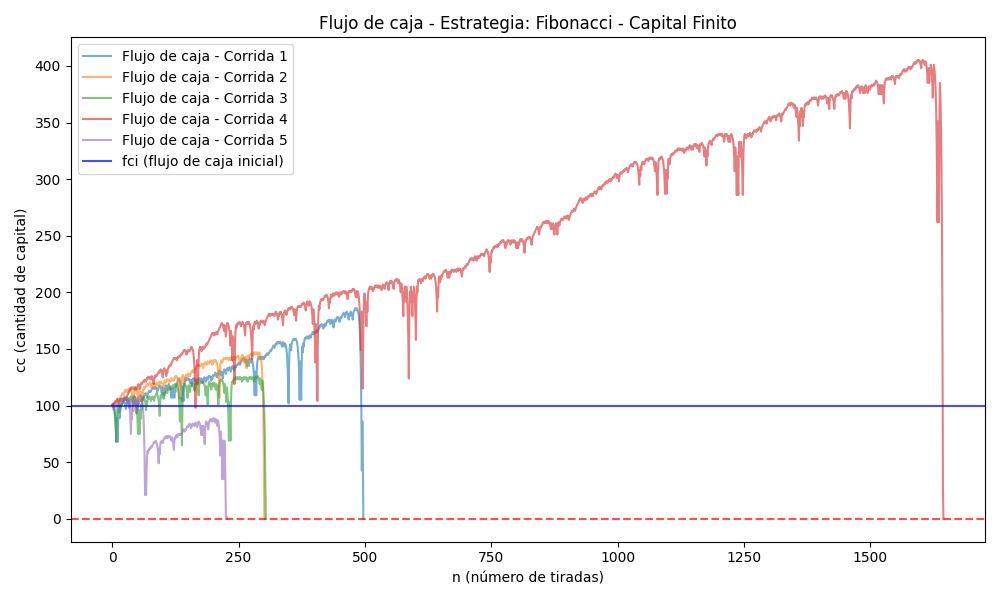
\includegraphics[width=0.7\linewidth]{Imagenes/flujo_caja_Fibonacci_f.png}
        \caption{Flujo de caja con capital finito}
        \label{fig:enter-label}
    \end{figure}
\end{itemize}

\begin{itemize}
    \item \textbf{Caja infinita:} Al eliminar la restricción del capital, la estrategia puede aplicarse indefinidamente. El flujo de caja evidencia oscilaciones cíclicas entre pérdidas y ganancias, manteniéndose relativamente más estable que en otros métodos progresivos. Aunque la recuperación tras rachas negativas suele ser efectiva, no se observa una tendencia claramente creciente en el capital, lo cual refleja que, incluso con capital ilimitado, la ventaja del casino termina afectando los resultados en el largo plazo.
\end{itemize}
\begin{figure}[H]
    \centering
    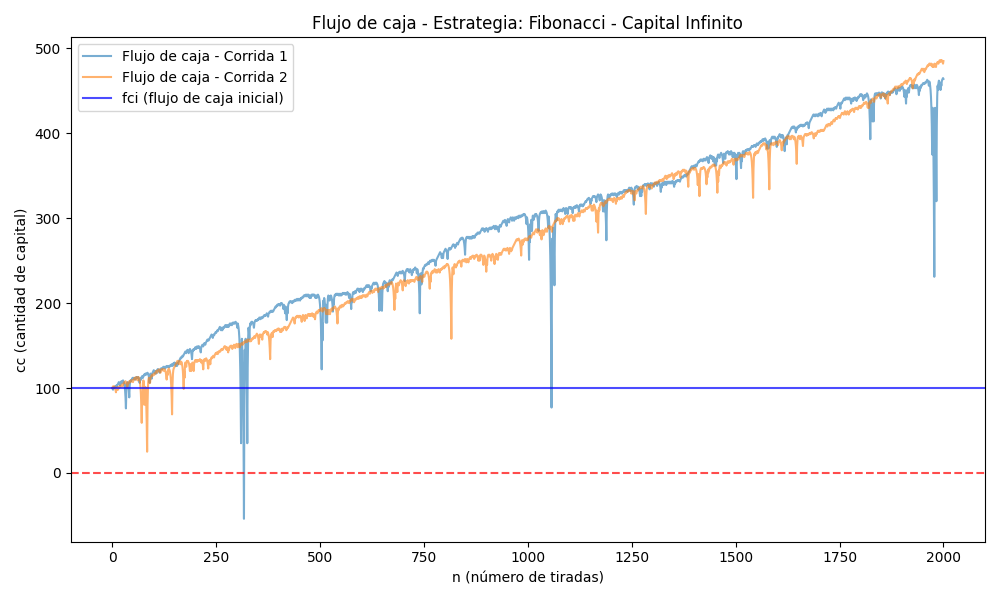
\includegraphics[width=0.7\linewidth]{Imagenes/flujo_caja_Fibonacci_i.png}
    \caption{Flujo de caja con capital infinito}
    \label{fig:enter-label}
\end{figure}

\subsubsection{Estrategia de Paroli}
La estrategia Paroli propone una lógica opuesta a la Martingala: en lugar de aumentar las apuestas tras una pérdida, se incrementan luego de cada victoria, aprovechando las rachas favorables. Esta progresión positiva tiene como objetivo maximizar ganancias limitando al mismo tiempo las pérdidas, ya que tras una derrota se reinicia la apuesta al valor base.

El análisis de frecuencias muestra, como en las demás estrategias, una estabilización progresiva de la frecuencia relativa acumulada hacia el valor teórico de 48.65\%. Las variaciones observadas en la frecuencia relativa por grupos de tiradas no muestran tendencias sistemáticas, reflejando un comportamiento propio de un sistema aleatorio como la ruleta.
\begin{figure}[H]
    \centering
    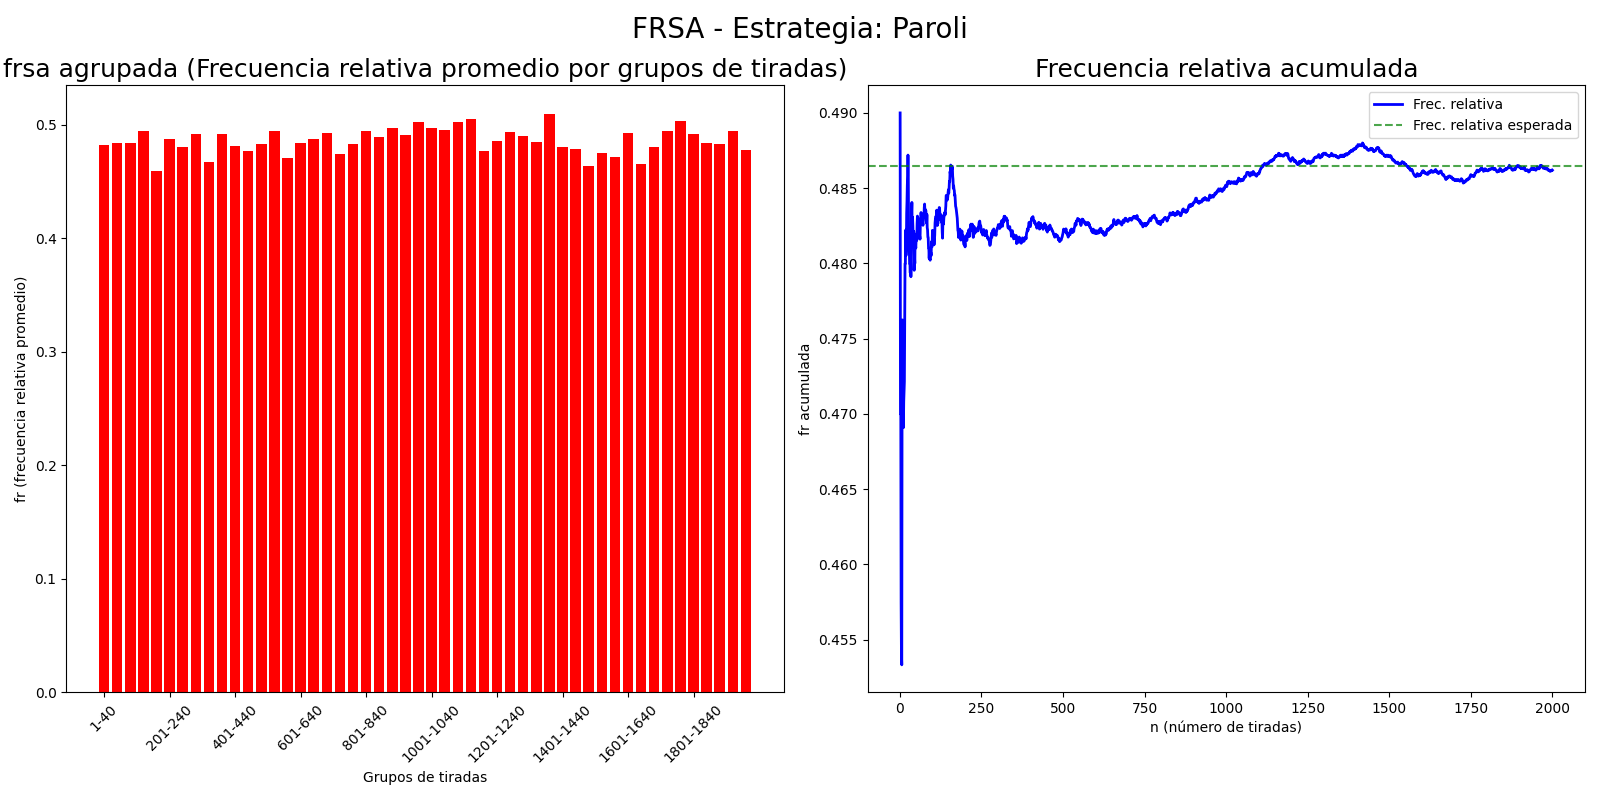
\includegraphics[width=1\linewidth]{Imagenes/frsa_Paroli.png}
    \caption{Frecuencia relativa promedio acumulada}
    \label{fig:paroli_finita}
\end{figure}

\begin{itemize}
    \item \textbf{Caja finita:} En este caso, el jugador dispone de un capital inicial limitado (100 unidades). La estrategia permite cierto crecimiento del capital en situaciones favorables, gracias a la acumulación de ganancias durante rachas positivas. Sin embargo, al depender de que dichas rachas ocurran dentro de un margen de apuestas controlado, se evidencia una vulnerabilidad frente a secuencias desfavorables. El flujo de caja resultante refleja oscilaciones cíclicas con algunas bancas rotas en distintas corridas simuladas.
\end{itemize}
\begin{figure}[H]
    \centering
    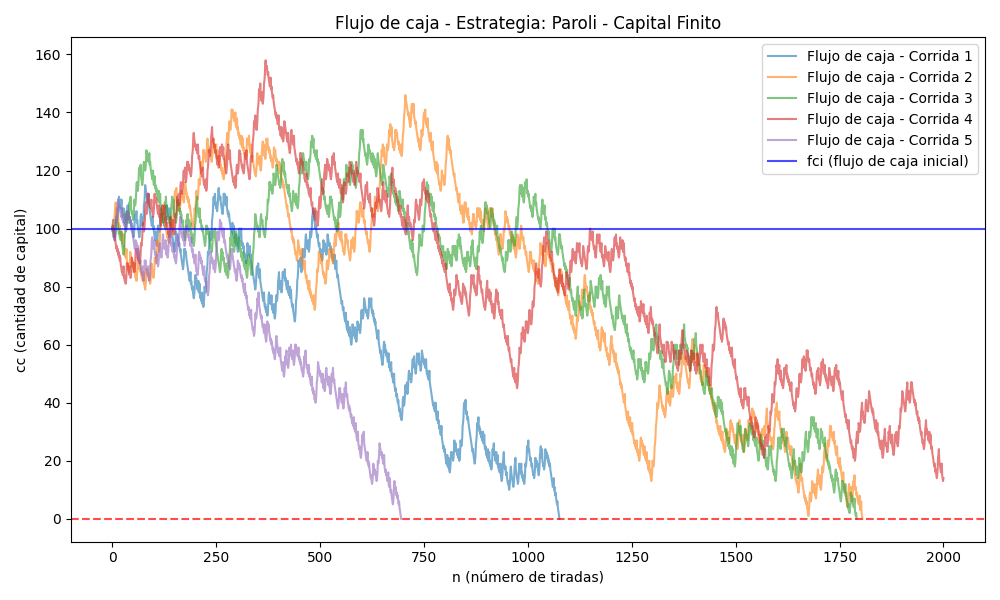
\includegraphics[width=0.7\linewidth]{Imagenes/flujo_caja_Paroli_f.png}
    \caption{Flujo de caja con capital finito}
    \label{fig:paroli_finita}
\end{figure}

\begin{itemize}
    \item \textbf{Caja infinita:}  Con capital ilimitado, el jugador puede aplicar la estrategia sin restricciones. El comportamiento observado en el flujo de caja conserva el carácter cíclico, con ganancias moderadas en fases favorables y descensos controlados en secuencias negativas. Si bien no se producen bancas rotas, tampoco se alcanza un crecimiento sostenido, mostrando que, aún en condiciones ideales, la estrategia no logra vencer la ventaja matemática del casino. 
\end{itemize}
    
\begin{figure}[H]
    \centering
    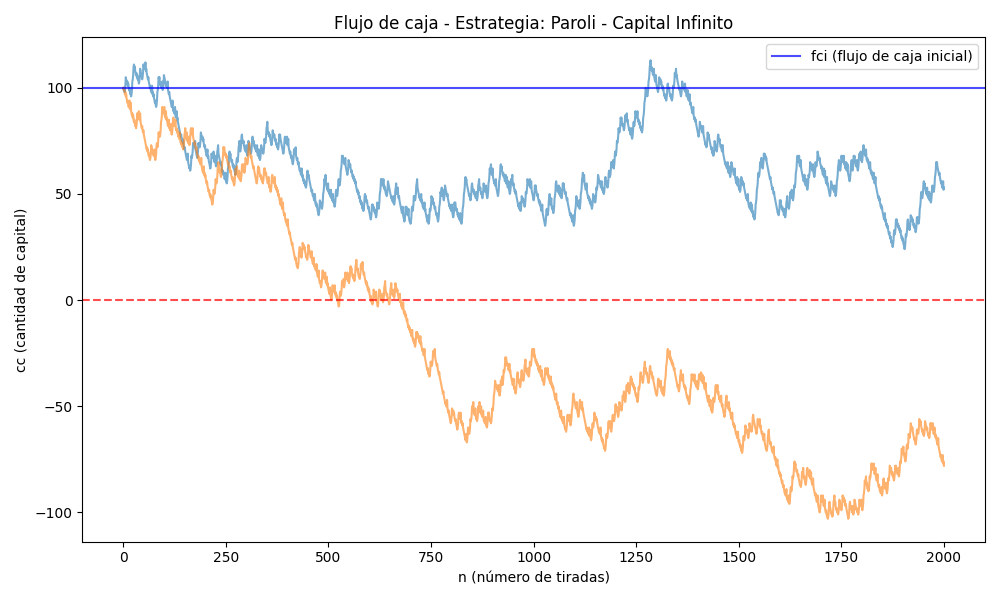
\includegraphics[width=0.7\linewidth]{Imagenes/flujo_caja_Paroli_i.png}
    \caption{Flujo de caja con capital infinito}
    \label{fig:paroli_inf}
\end{figure}        

\section{Conclusión}
A lo largo de este trabajo, analizamos y simulamos distintas estrategias de apuestas aplicadas a la ruleta bajo dos escenarios contrastantes: capital finito e infinito. Cada sistema de apuestas mostró comportamientos característicos que permitieron evaluar sus fortalezas, limitaciones y riesgos asociados.

Se observó que, si bien algunas estrategias permiten una mejor gestión del capital en el corto plazo (como Fibonacci o D'Alembert), ninguna elimina la ventaja estadística de la casa.

Si bien la simulación con capital infinito nos ayuda a comprender el comportamiento ideal de las estrategias, en la práctica siempre estamos limitados por el dinero real disponible. Esto evidencia que muchas estrategias que parecen efectivas en teoría no son viables en situaciones reales, donde quedarse sin fondos es un riesgo concreto.

El análisis gráfico permitió visualizar fenómenos como la estabilización de la frecuencia relativa hacia los valores teóricos esperados, el impacto de las rachas de pérdidas en estrategias progresivas como la Martingala, y la moderación que introduce Fibonacci frente a apuestas más agresivas.

Es evidente que, independientemente del sistema de apuestas empleado, la ruleta sigue siendo un juego de azar puro, donde las leyes matemáticas no pueden prever el resultado ni garantizar ganancias consistentes. La imprevisibilidad inherente del juego deja en claro que cada giro de la rueda es completamente aleatorio e impredecible.

\bibliographystyle{unsrt}  
\begin{thebibliography}

\bibitem{simulaciongithub}
Aldana Risso Patrón. \textit{TP 1.2 - Estudio Económico-Matemático de apuestas en la Ruleta (código fuente)}.\\
Disponible en: \url{https://github.com/AldanaRP/TPSimulacion} \\

\bibitem{bacchini2018}
Bacchini, H. \textit{Introducción a la Probabilidad y a la Estadística}.\\
Universidad de Buenos Aires, Facultad de Ciencias Económicas, 2018.\\
Disponible en: \url{http://bibliotecadigital.econ.uba.ar/download/libros/Bacchini_Introduccion-a-la-probabilidad-y-a-la-estadistica-2018.pdf}

\end{thebibliography}

    
\end{document}
